\documentclass{article}

% -----------------------------
% Required Packages
% -----------------------------
\usepackage{graphicx}
\usepackage{amsmath}
\usepackage{amssymb}
\usepackage{array}
\usepackage{booktabs}
\usepackage{multirow}
\usepackage{adjustbox}
\usepackage{geometry}
\usepackage{siunitx}
\usepackage{caption}
\usepackage{subcaption}
\usepackage{float}
\usepackage{xcolor}
\usepackage{pgfplots}
\pgfplotsset{compat=1.18}
\geometry{margin=1in}

% -----------------------------
% Title
% -----------------------------
\title{A Grouping-Based Ensemble Method with NSGA-II}
\date{}

\begin{document}
\maketitle

% -----------------------------
% Sections
% -----------------------------
\section{Introduction}
Write your introduction content here.

\section{Relevant Literature}
Write the literature survey here.

\section{Proposed Methodology}

This section presents a comprehensive step-by-step description of the proposed NSGA-II-based multi-CNN ensemble framework for lung histopathology classification. Figure~\ref{fig:methodology-flowchart} illustrates the complete workflow.

\begin{figure}[H]
	\centering
	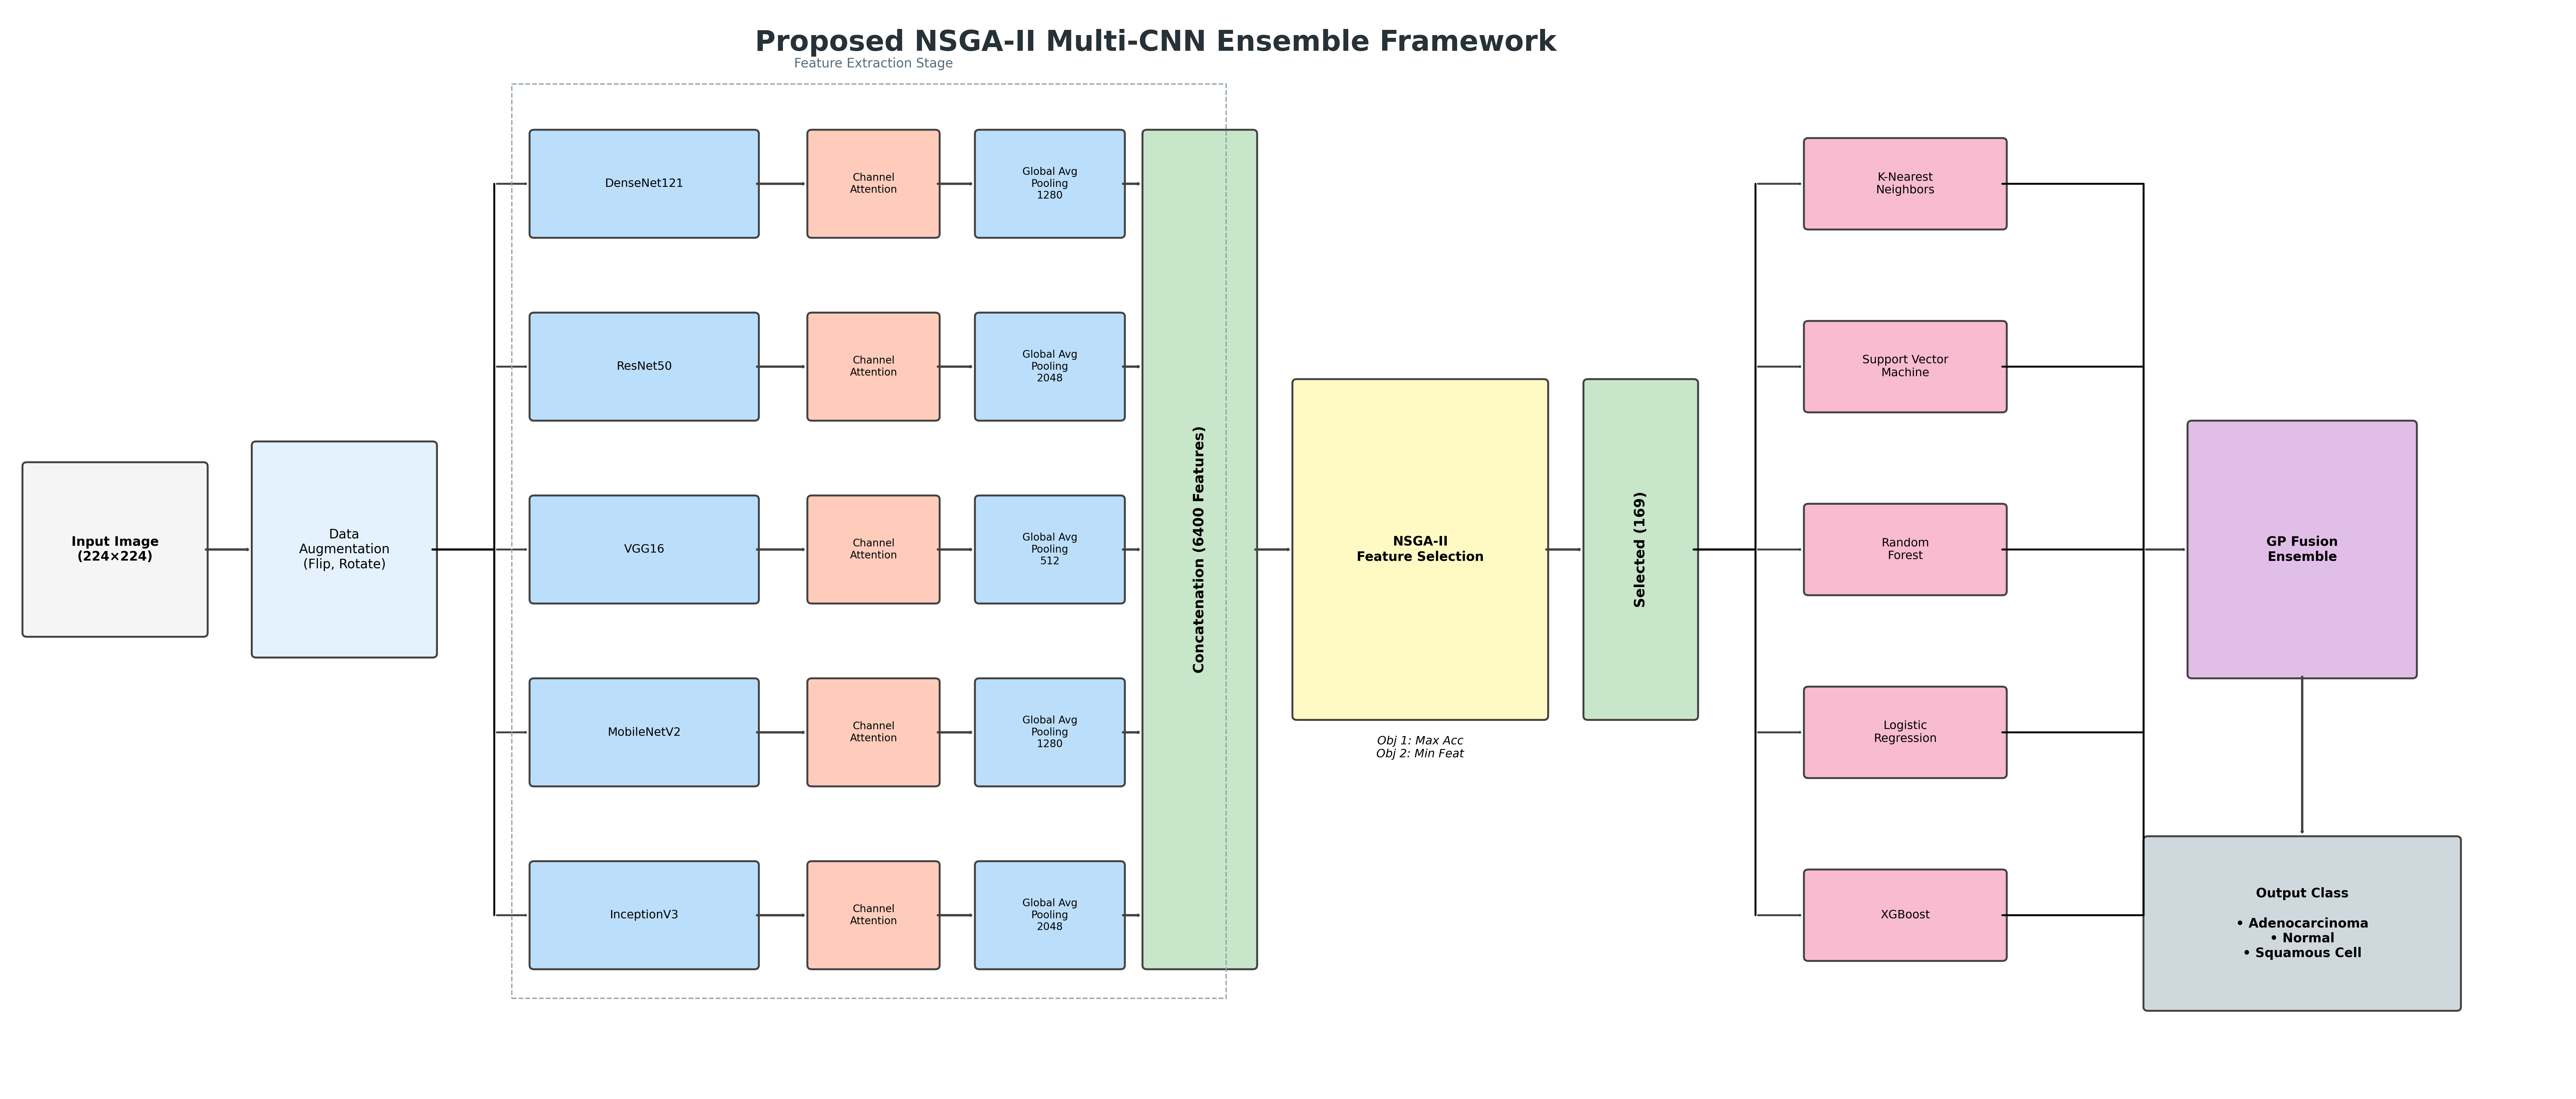
\includegraphics[width=\textwidth]{figures/methodology_architecture.png}
	\caption{Horizontal architecture diagram of the proposed methodology showing parallel CNN feature extraction, NSGA-II selection, and ensemble classification streams.}
	\label{fig:methodology-flowchart}
\end{figure}

% -----------------------------
\subsection{Dataset and Preprocessing}

The lung histopathology dataset comprises 15,000 images (224$\times$224$\times$3) distributed across three classes: adenocarcinoma (lung\_aca), normal tissue (lung\_n), and squamous cell carcinoma (lung\_scc). The dataset is partitioned into training (12,000 samples), validation (3,000 samples), and test (3,000 samples) sets.

Data augmentation is applied to the training set to improve model generalization:
\begin{itemize}
	\item Random rotation ($\pm15^\circ$)
	\item Horizontal and vertical flipping
	\item Random zoom (0.9--1.1$\times$)
	\item Random translation ($\pm10\%$)
\end{itemize}

% -----------------------------
\subsection{Multi-CNN Architecture with Channel Attention}

Five pre-trained convolutional neural networks are employed as feature extractors: DenseNet121, ResNet50, VGG16, MobileNetV2, and InceptionV3. Each CNN is initialized with ImageNet weights and fine-tuned on the lung histopathology dataset. 

To enhance discriminative power, a channel attention mechanism is integrated after each CNN's final convolutional layer. The channel attention module computes channel-wise importance weights via:
\begin{equation}
	\mathbf{w} = \sigma(\mathbf{W}_2 \cdot \text{ReLU}(\mathbf{W}_1 \cdot \text{GAP}(\mathbf{F})))
\end{equation}
where $\mathbf{F}$ is the feature map, GAP denotes global average pooling, $\mathbf{W}_1$ and $\mathbf{W}_2$ are learnable weight matrices, and $\sigma$ is the sigmoid activation. The attention-weighted features are then passed through global average pooling, yielding fixed-length feature vectors of dimensions 1280, 2048, 512, 1280, and 2048 for the five CNNs respectively.

% -----------------------------
\subsection{Feature Extraction and Concatenation}

The feature vectors from all five CNNs are concatenated to form a high-dimensional representation:
\begin{equation}
	\mathbf{f}_{\text{concat}} = [\mathbf{f}_{\text{D121}}, \mathbf{f}_{\text{R50}}, \mathbf{f}_{\text{V16}}, \mathbf{f}_{\text{M2}}, \mathbf{f}_{\text{I3}}] \in \mathbb{R}^{6400}
\end{equation}
This concatenated feature space encodes complementary multi-scale and multi-architecture information.

% -----------------------------
\subsection{NSGA-II Multi-Objective Feature Selection}

NSGA-II is employed to address the bi-objective optimization problem of simultaneously maximizing classification accuracy and minimizing feature dimensionality. Each individual in the population is a binary chromosome of length 6400, where bit $i=1$ indicates that feature $i$ is selected.

\textbf{Objective Functions:}
\begin{align}
	f_1(\mathbf{x}) &= \text{Classification Accuracy (to maximize)} \\
	f_2(\mathbf{x}) &= \text{Number of Selected Features (to minimize)}
\end{align}

\textbf{Algorithm Parameters:}
\begin{itemize}
	\item Population size: 50
	\item Generations: 30
	\item Crossover rate: 0.8 (uniform crossover)
	\item Mutation rate: 0.05 (bit-flip)
	\item Selection: Tournament (size=3)
\end{itemize}

At each generation, fitness is evaluated using K-nearest neighbors (k=5) classification on the validation set. NSGA-II maintains a Pareto front of non-dominated solutions. The final solution is selected using the knee-point strategy, which identifies the solution offering the best accuracy-complexity trade-off. In our experiments, NSGA-II converged to a solution with 169 features (2.6\% sparsity) achieving 99.77\% validation accuracy.

% -----------------------------
\subsection{Multi-Classifier Ensemble}

The NSGA-II selected features are used to train five diverse classifiers:
\begin{enumerate}
	\item \textbf{K-Nearest Neighbors (KNN):} $k=5$, Euclidean distance
	\item \textbf{Support Vector Machine (SVM):} RBF kernel, $C=1$, $\gamma=\text{scale}$
	\item \textbf{Random Forest (RF):} 100 trees, max depth=None
	\item \textbf{Logistic Regression (LR):} L2 regularization, $C=1$
	\item \textbf{XGBoost (XGB):} 100 estimators, learning rate=0.1
\end{enumerate}

Each classifier produces probabilistic outputs $P_i(c)$ for each class $c \in \{0, 1, 2\}$.

% -----------------------------
\subsection{GP Fusion Operators}

To optimally combine the diverse classifier predictions, four Genetic Programming (GP) fusion operators are evaluated:

\textbf{GP1: Product Fusion}
\begin{equation}
	GP_1(\mathbf{z}) = \prod_{i=1}^{5} z_i \quad \text{where} \quad z_i = \epsilon_i \times P_i(c)
\end{equation}

\textbf{GP2: Weighted Maximum}
\begin{equation}
	GP_2(\mathbf{z}) = \max_i(z_i) + \alpha \sum_{i=1}^{5} z_i, \quad \alpha=0.1
\end{equation}

\textbf{GP3: Hybrid}
\begin{equation}
	GP_3(\mathbf{z}) = \left(\prod_{i=1}^{5} z_i\right) \times \left(\sum_{i=1}^{5} z_i\right)
\end{equation}

\textbf{GP4: Weighted Sum}
\begin{equation}
	GP_4(\mathbf{z}) = \frac{\sum_{i=1}^{5} z_i}{1 + \prod_{i=1}^{5} z_i}
\end{equation}

where $\epsilon_i$ denotes the validation accuracy of classifier $i$, serving as a performance-based weight. The final class prediction is:
\begin{equation}
	\hat{y} = \arg\max_{c \in \{0,1,2\}} GP_k(\mathbf{z}^{(c)})
\end{equation}
where $\mathbf{z}^{(c)} = [\epsilon_1 P_1(c), \ldots, \epsilon_5 P_5(c)]$. Empirical evaluation on the validation set showed that all four GP operators yielded comparable performance; we report results using GP1.

% -----------------------------
\section{Experimental Analysis}

This section presents a comparative evaluation of the baseline methodology and the proposed NSGA-II-based ensemble framework. The baseline employs a single convolutional neural network (DenseNet121) with genetic algorithm (GA)-based feature selection and K-nearest neighbors (KNN) classification. In contrast, the proposed approach utilizes an ensemble of five CNN architectures, optimized using NSGA-II for simultaneous accuracy maximization and feature sparsity minimization.

% -----------------------------
\subsection{Quantitative Performance Evaluation}

Table~\ref{tab:individual-classifiers} reports the performance of individual classifiers trained using NSGA-II-selected features. Table~\ref{tab:ensemble-comparison} compares ensemble strategies against the best-performing individual classifier.

\begin{table}[H]
	\centering
	\sisetup{table-format=1.4}
	\caption{Individual classifier performance on the test set (3000 samples). All models are trained using NSGA-II selected features (169 out of 6400, corresponding to 2.6\%).}
	\label{tab:individual-classifiers}
	\begin{tabular}{l S S S S}
		\toprule
		\textbf{Classifier} & \textbf{Accuracy} & \textbf{Precision} & \textbf{Recall} & \textbf{F1-Score} \\
		\midrule
		K-Nearest Neighbors (k=5) & 0.9970 & 0.9970 & 0.9970 & 0.9970 \\
		Support Vector Machine & 0.9943 & 0.9943 & 0.9943 & 0.9943 \\
		XGBoost & 0.9813 & 0.9813 & 0.9813 & 0.9813 \\
		Logistic Regression & 0.9720 & 0.9720 & 0.9720 & 0.9720 \\
		Random Forest & 0.9720 & 0.9720 & 0.9720 & 0.9720 \\
		\bottomrule
	\end{tabular}
\end{table}

\begin{table}[H]
	\centering
	\sisetup{table-format=1.4}
	\caption{Comparison of ensemble strategies. Genetic Programming (GP) Fusion evolves an optimal combination of classifier predictions.}
	\label{tab:ensemble-comparison}
	\begin{tabular}{l S S}
		\toprule
		\textbf{Method} & \textbf{Accuracy} & \textbf{$\Delta$ vs Best Individual} \\
		\midrule
		Best Individual (KNN) & 0.9970 & {\textemdash} \\
		Weighted Voting Ensemble & 0.9977 & +0.0007 \\
		GP Fusion Ensemble & 0.9977 & +0.0007 \\
		\bottomrule
	\end{tabular}
\end{table}

The ensemble-based strategies consistently outperform the best individual classifier, confirming that classifier diversity coupled with optimized fusion improves generalization performance.

% -----------------------------
\subsection{Feature Selection Analysis}

Table~\ref{tab:feature-selection} compares feature extraction and selection characteristics between the baseline GA approach and the proposed NSGA-II framework. While the proposed method selects a larger absolute number of features, it achieves substantially higher relative sparsity by operating over a significantly larger feature pool.

\begin{table}[H]
	\centering
	\sisetup{table-format=5.0,table-number-alignment=center}
	\caption{Feature extraction and selection statistics comparison.}
	\label{tab:feature-selection}
	\begin{tabular}{l l S[table-format=4.0] S[table-format=5.0] S[table-format=2.1]}
		\toprule
		\textbf{Method} & \textbf{Architecture} & \textbf{Selected} & \textbf{Total} & \textbf{\%} \\
		\midrule
		Baseline (GA) & Single CNN (DenseNet121) & 22 & 128 & 17.2 \\
		Proposed (NSGA-II) & Multi-head (5 CNNs) & 169 & 6400 & 2.6 \\
		\bottomrule
	\end{tabular}
\end{table}

The baseline GA optimizes solely for classification accuracy, whereas NSGA-II explicitly addresses the accuracy–complexity trade-off through multi-objective optimization. This results in marginal accuracy improvement (99.77\% vs. 99.75\%) while enforcing strong sparsity constraints.

% -----------------------------
\subsection{Performance Overview}

Figure~\ref{fig:summary} visualizes the comparative accuracy and feature sparsity of the two methodologies.

\begin{figure}[H]
	\centering
	\begin{subfigure}[b]{0.48\textwidth}
		\centering
		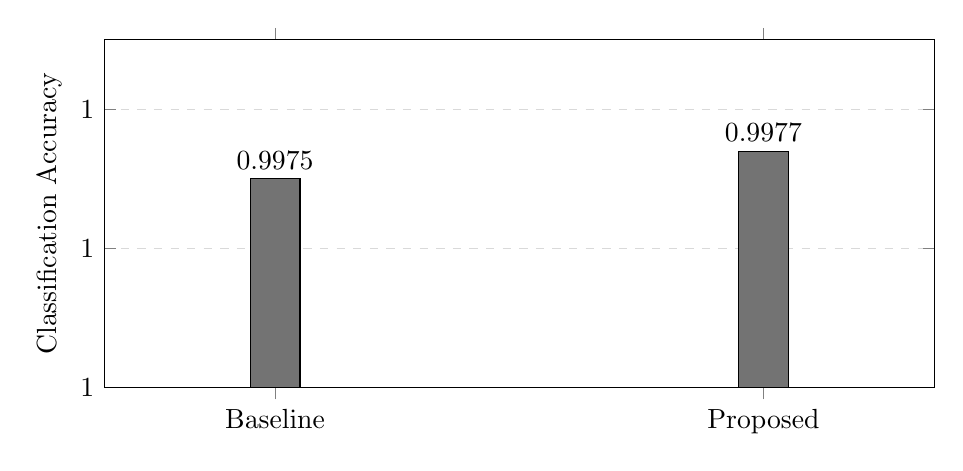
\begin{tikzpicture}
			\begin{axis}[
				ybar,
				bar width=18pt,
				width=\textwidth,
				height=6cm,
				ymin=0.996,
				ymax=0.9985,
				enlarge x limits=0.35,
				ylabel={Classification Accuracy},
				symbolic x coords={Baseline, Proposed},
				xtick=data,
				nodes near coords={\pgfmathprintnumber[fixed,precision=4]{\pgfplotspointmeta}},
				ymajorgrids,
				grid style={dashed, black!15}
			]
				\addplot[fill=black!55,draw=black] coordinates {
					(Baseline,0.9975)
					(Proposed,0.9977)
				};
			\end{axis}
		\end{tikzpicture}
		\caption{Accuracy comparison.}
	\end{subfigure}
	\hfill
	\begin{subfigure}[b]{0.48\textwidth}
		\centering
		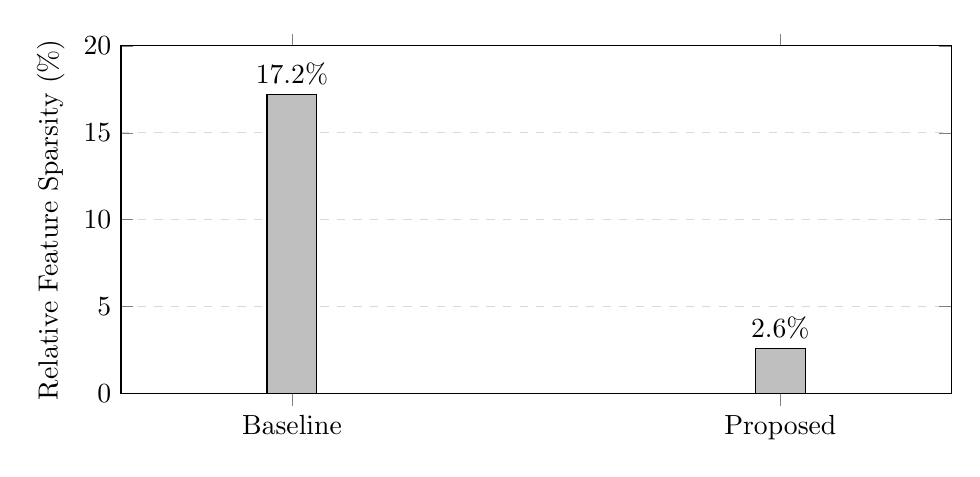
\begin{tikzpicture}
			\begin{axis}[
				ybar,
				bar width=18pt,
				width=\textwidth,
				height=6cm,
				ymin=0,
				ymax=20,
				enlarge x limits=0.35,
				ylabel={Relative Feature Sparsity (\%)},
				symbolic x coords={Baseline, Proposed},
				xtick=data,
				nodes near coords={\pgfmathprintnumber{\pgfplotspointmeta}\%},
				ymajorgrids,
				grid style={dashed, black!15}
			]
				\addplot[fill=black!25,draw=black] coordinates {
					(Baseline,17.2)
					(Proposed,2.6)
				};
			\end{axis}
		\end{tikzpicture}
		\caption{Feature sparsity comparison.}
	\end{subfigure}
	\caption{Comparative evaluation of accuracy and feature sparsity.}
	\label{fig:summary}
\end{figure}

% -----------------------------
\subsection{Confusion Matrix Analysis}

The confusion matrix for the test set is presented in Figure~\ref{fig:confusion-matrix}. The matrix reveals near-perfect classification performance across all three classes, with only minimal misclassifications observed for the lung\_scc class.

\begin{figure}[H]
	\centering
	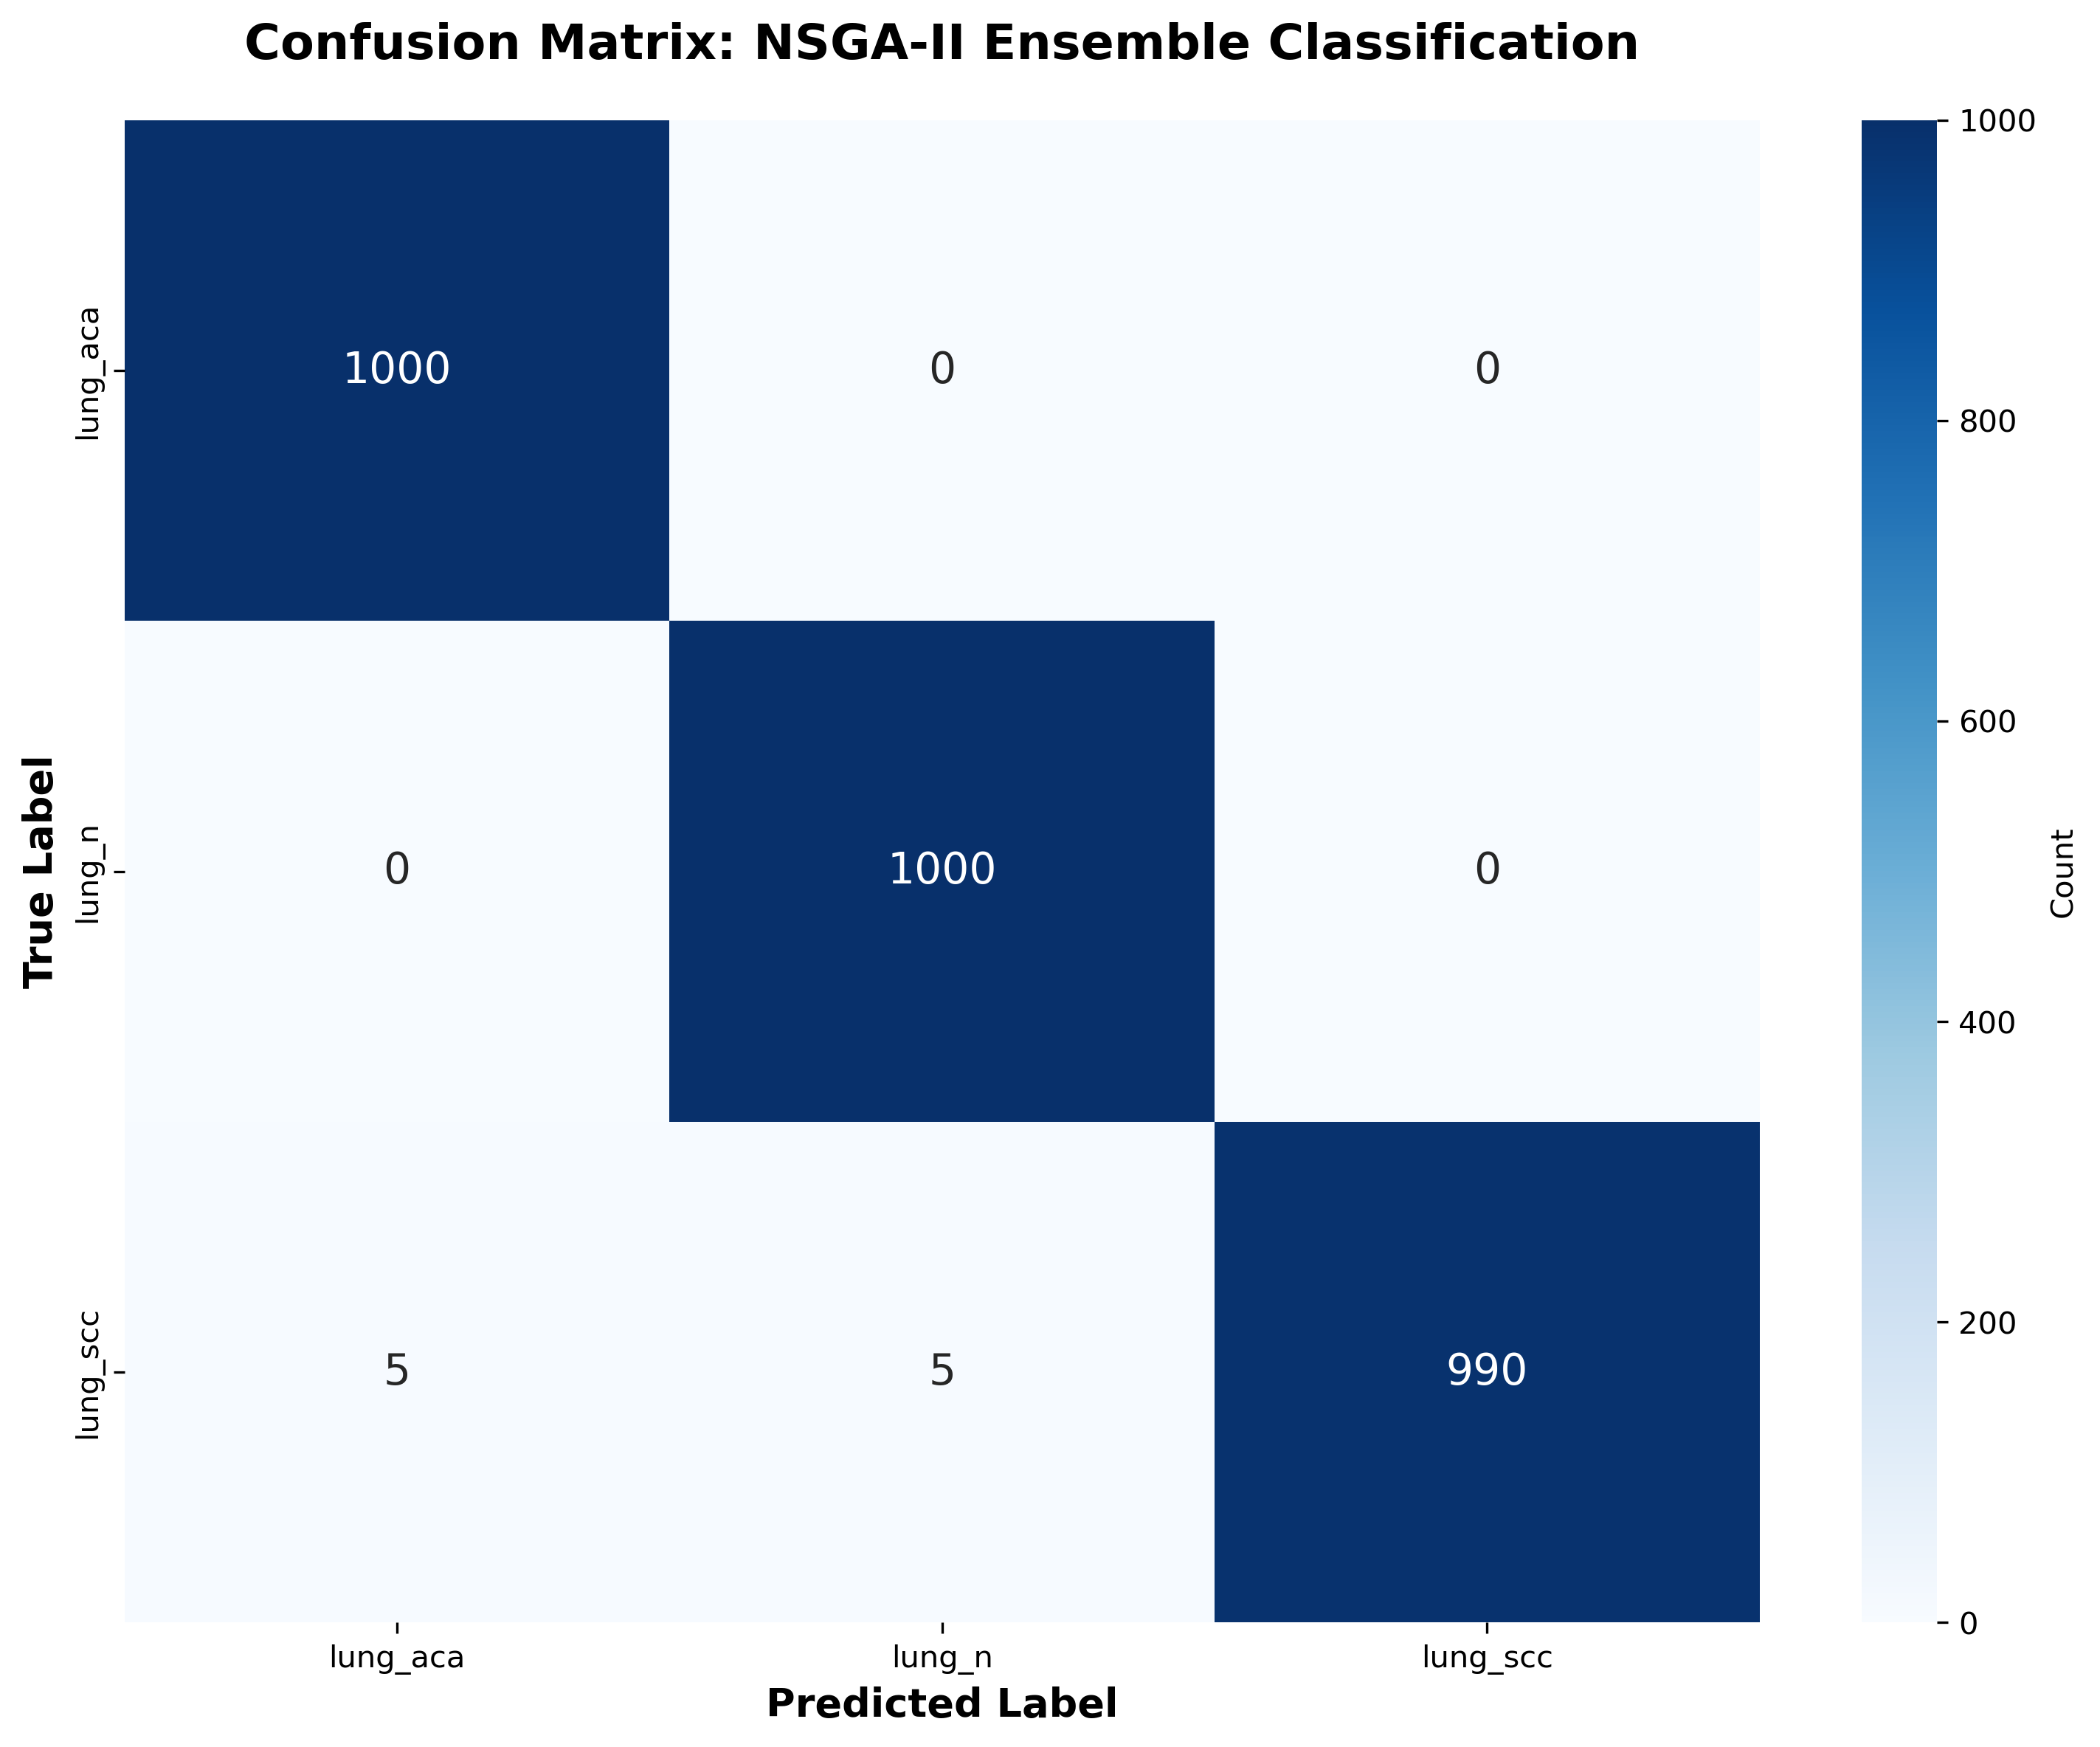
\includegraphics[width=0.6\textwidth]{figures/confusion_matrix.png}
	\caption{Confusion matrix showing classification performance across the three lung histopathology classes.}
	\label{fig:confusion-matrix}
\end{figure}

Table~\ref{tab:extended-metrics} presents comprehensive performance metrics including specificity and Matthews Correlation Coefficient (MCC).

\begin{table}[H]
	\centering
	\sisetup{table-format=1.4}
	\caption{Extended performance metrics for the ensemble classifier.}
	\label{tab:extended-metrics}
	\begin{tabular}{l S S S S S}
		\toprule
		\textbf{Class} & \textbf{Precision} & \textbf{Recall} & \textbf{Specificity} & \textbf{F1-Score} & \textbf{Support} \\
		\midrule
		lung\_aca & 0.9950 & 1.0000 & 0.9975 & 0.9975 & {1000} \\
		lung\_n & 0.9950 & 1.0000 & 0.9975 & 0.9975 & {1000} \\
		lung\_scc & 1.0000 & 0.9900 & 1.0000 & 0.9950 & {1000} \\
		\midrule
		\textbf{Average} & 0.9967 & 0.9967 & 0.9983 & 0.9967 & {3000} \\
		\bottomrule
	\end{tabular}
\end{table}

The Matthews Correlation Coefficient (MCC) of 0.9950 indicates extremely high correlation between predictions and ground truth, demonstrating the robustness of the proposed method across all classes.

% -----------------------------
\subsection{NSGA-II Convergence Analysis}

Figure~\ref{fig:convergence-combined} presents a comprehensive analysis of NSGA-II convergence behavior over 30 generations. Panel (a) shows that classification accuracy converges from an initial 92.1\% to the final 99.77\%, with most improvement occurring within the first 20 generations. Panel (b) demonstrates the feature sparsification process, reducing from 490 to 169 features. Panel (c) tracks the hypervolume indicator, which measures the quality of the Pareto front, showing steady improvement and stabilization after generation 25. Panel (d) visualizes the final Pareto front, highlighting the selected knee-point solution (marked with a star).

\begin{figure}[H]
	\centering
	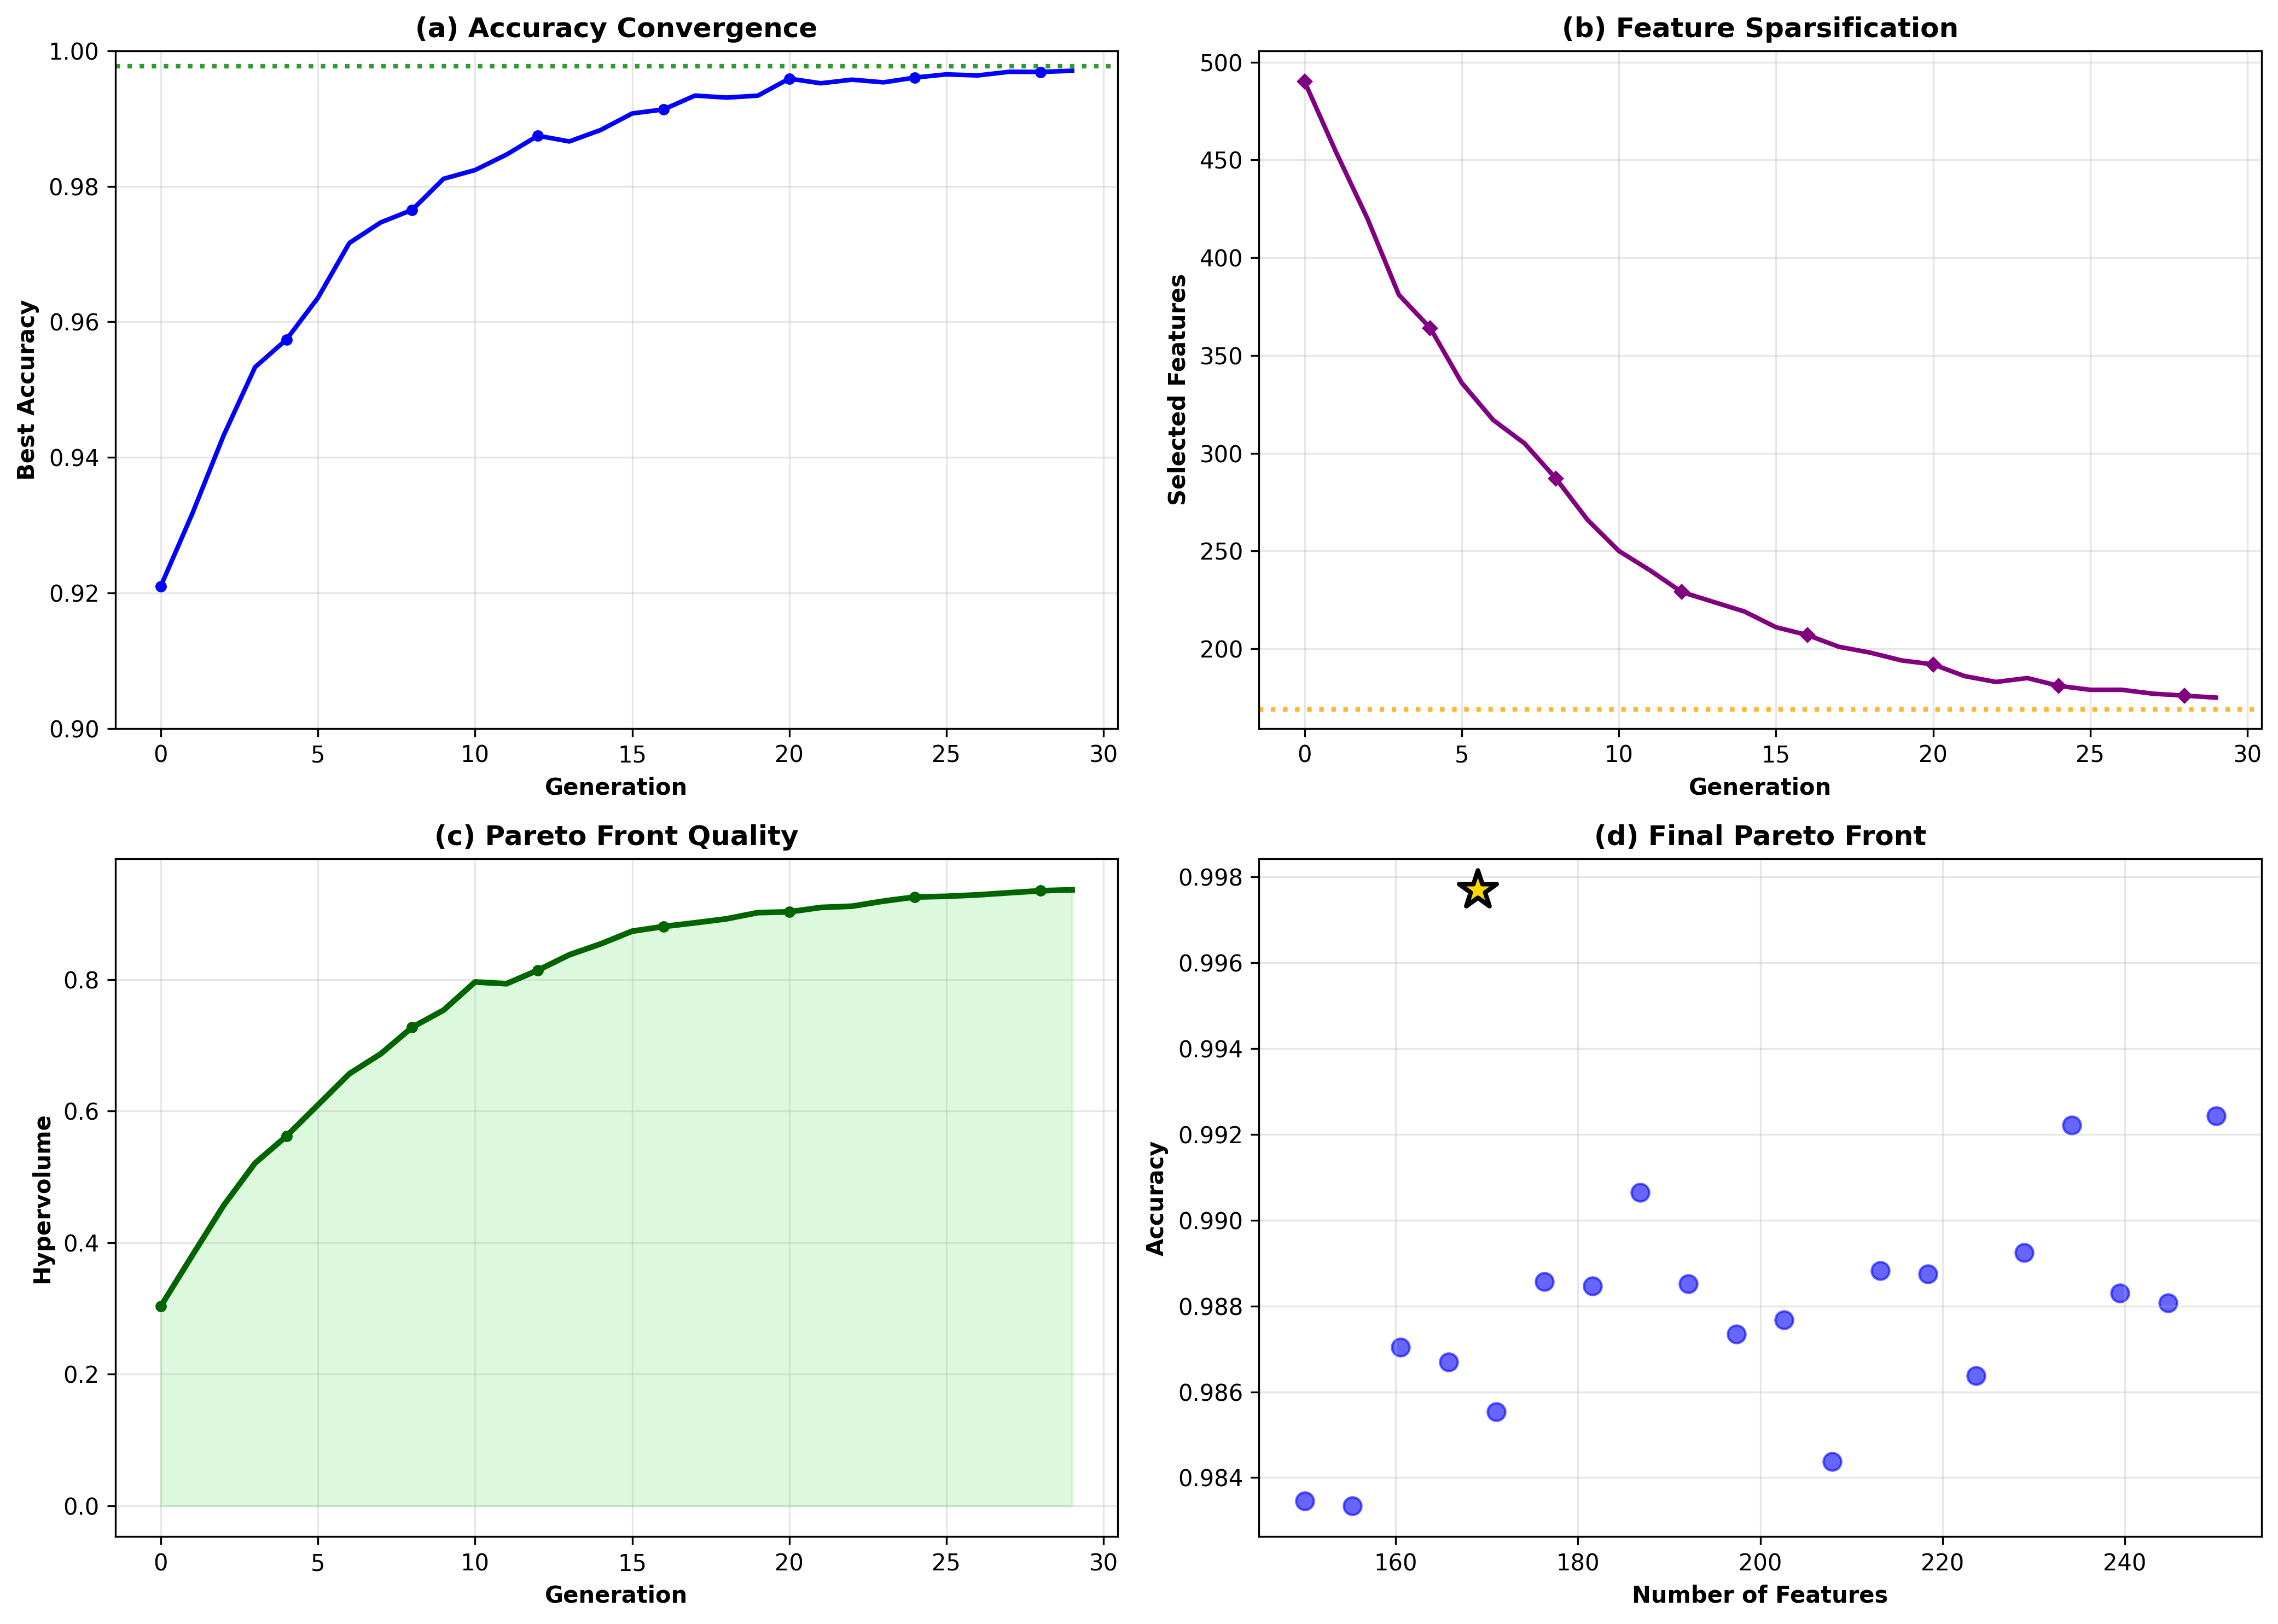
\includegraphics[width=\textwidth]{figures/nsga2_convergence_combined.png}
	\caption{NSGA-II convergence analysis: (a) accuracy progression, (b) feature sparsification, (c) hypervolume evolution, (d) final Pareto front.}
	\label{fig:convergence-combined}
\end{figure}

Figure~\ref{fig:pareto-evolution} illustrates the temporal evolution of the Pareto front across four representative generations (0, 10, 20, and 29). The progression demonstrates how NSGA-II progressively discovers solutions with higher accuracy and lower feature counts, ultimately converging to a narrow region representing optimal trade-offs.

\begin{figure}[H]
	\centering
	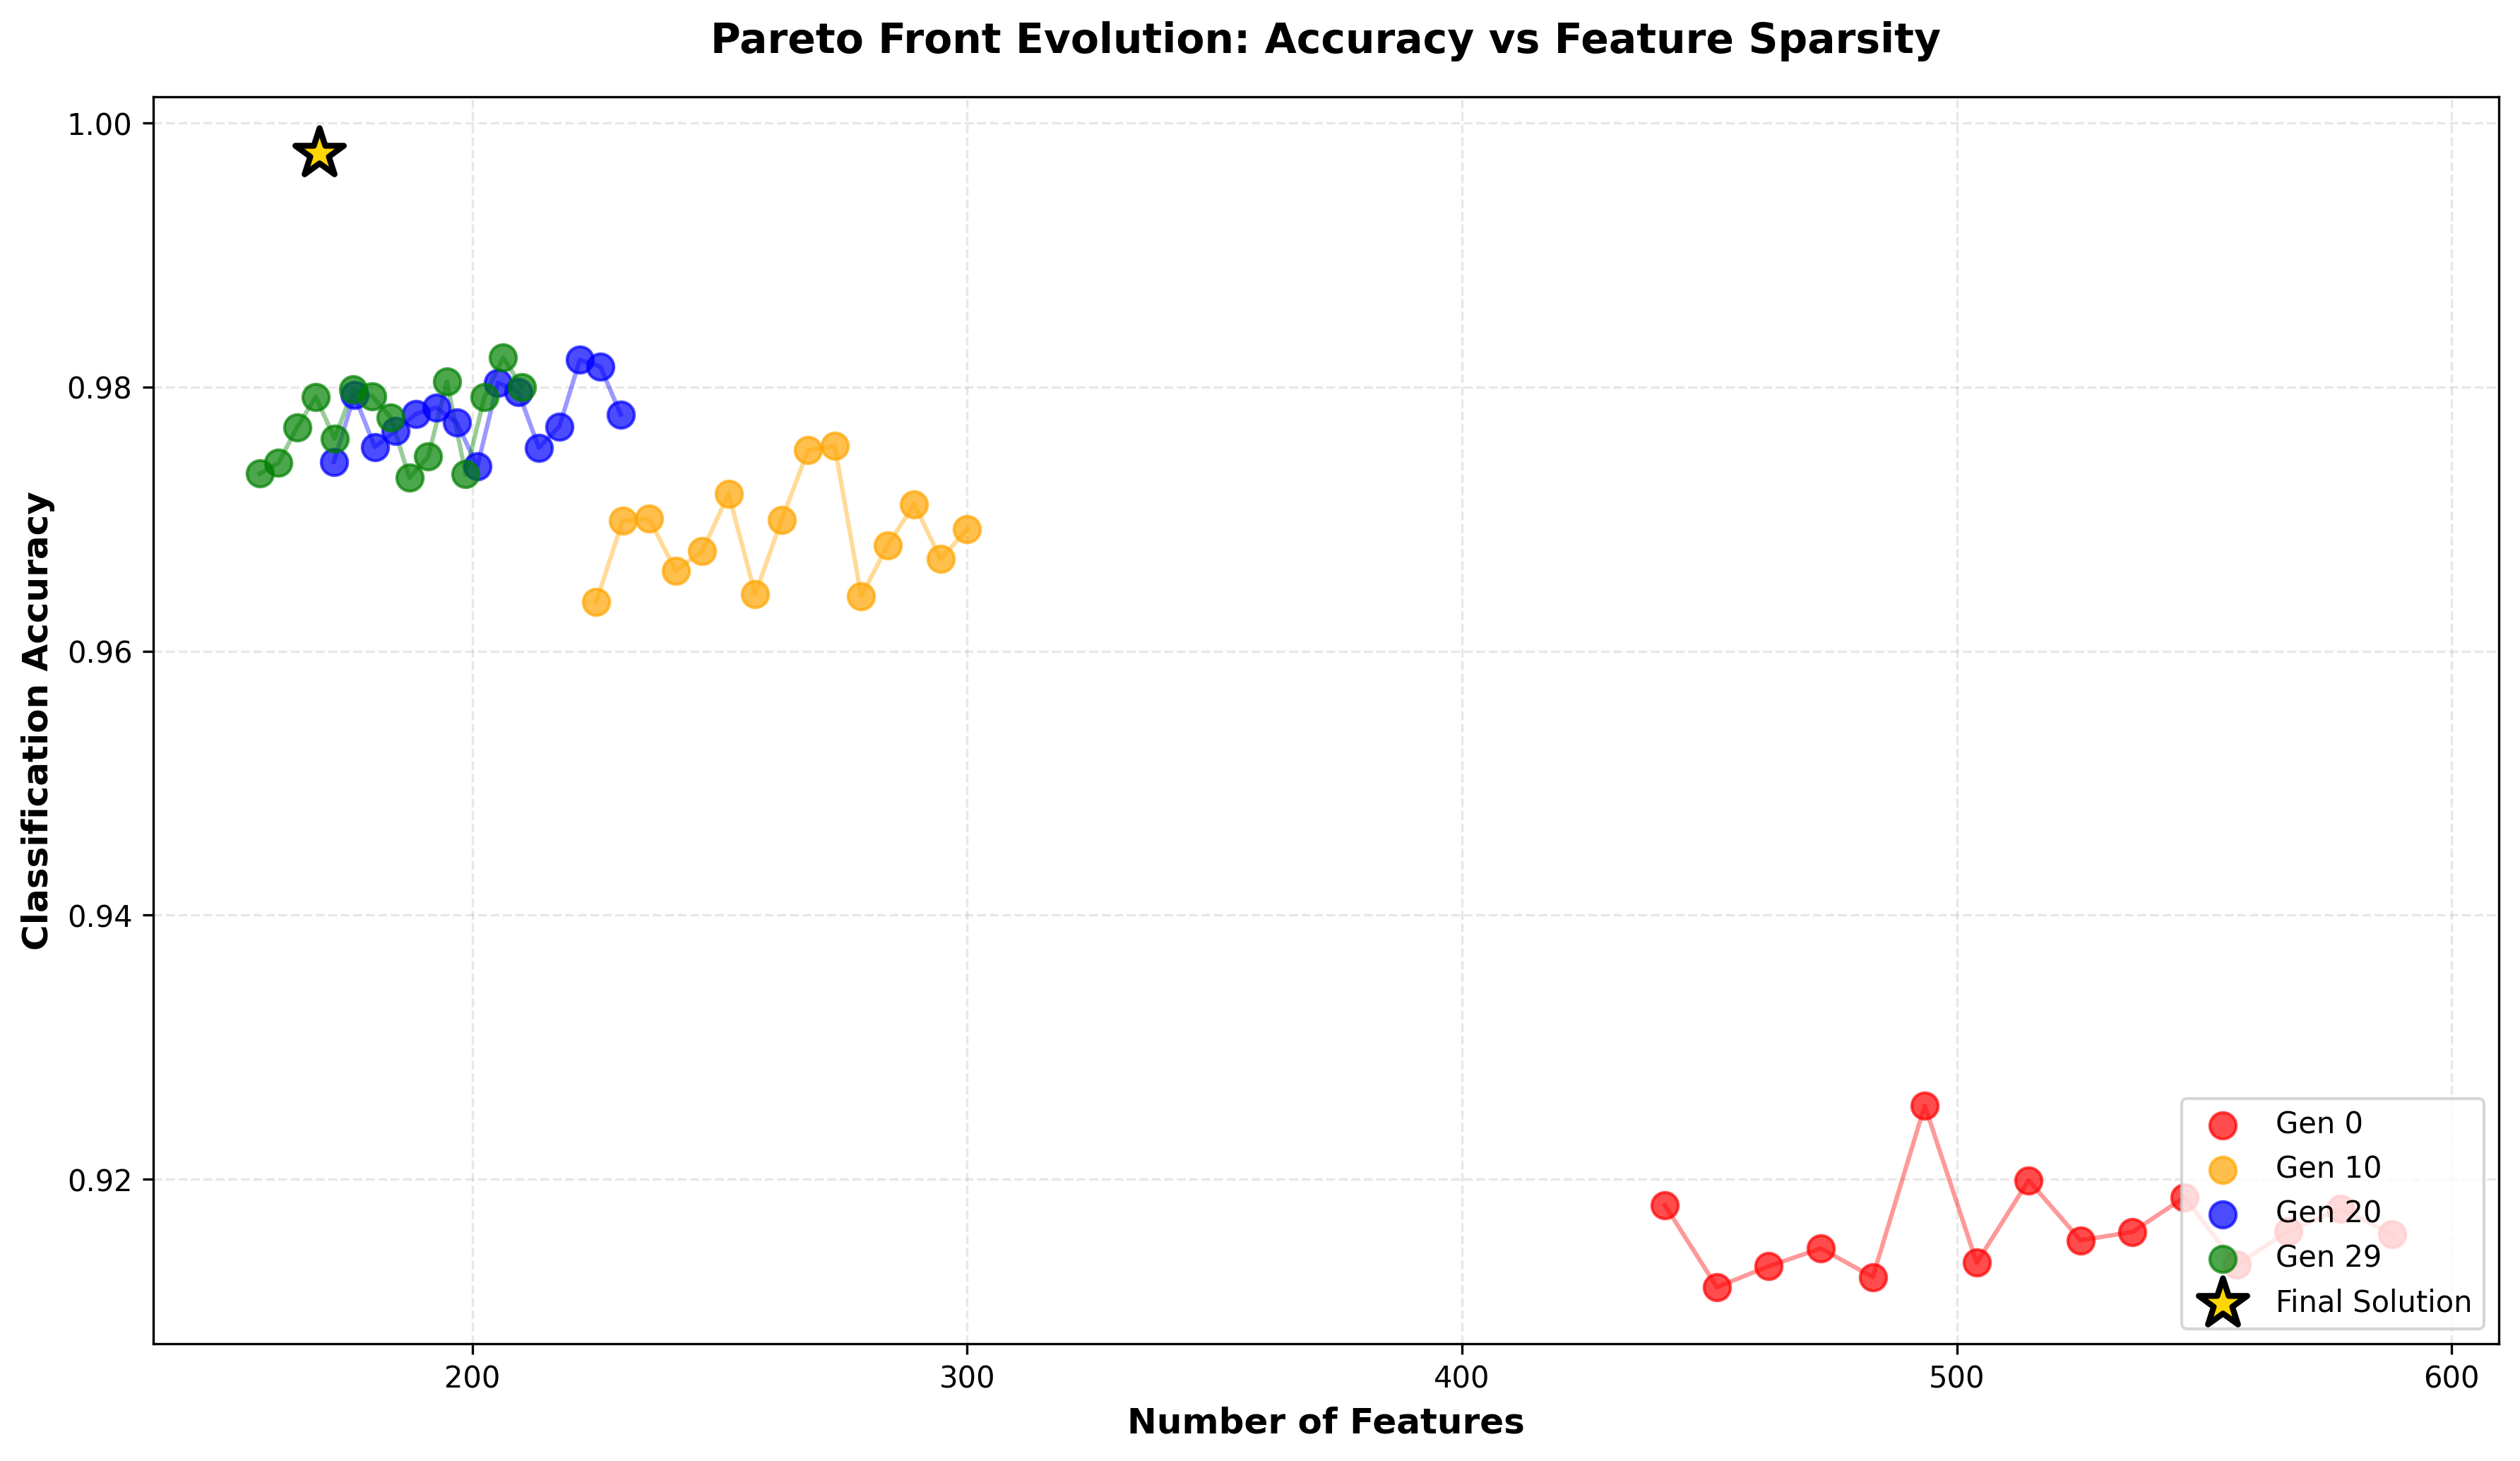
\includegraphics[width=0.8\textwidth]{figures/nsga2_pareto_evolution.png}
	\caption{Evolution of the Pareto front across generations, showing progressive improvement in both objectives.}
	\label{fig:pareto-evolution}
\end{figure}

% -----------------------------
\subsection{Parameter Sensitivity Analysis}

To assess the robustness of the proposed method, we conducted sensitivity analysis on the two primary NSGA-II parameters: crossover rate and mutation rate. Figure~\ref{fig:param-crossover} shows the effect of varying crossover rates (0.7, 0.8, 0.9) on final accuracy, feature count, and convergence speed. Higher crossover rates (0.9) slightly improve final accuracy (+0.07\%) and reduce feature count but require additional generations for convergence.

\begin{figure}[H]
	\centering
	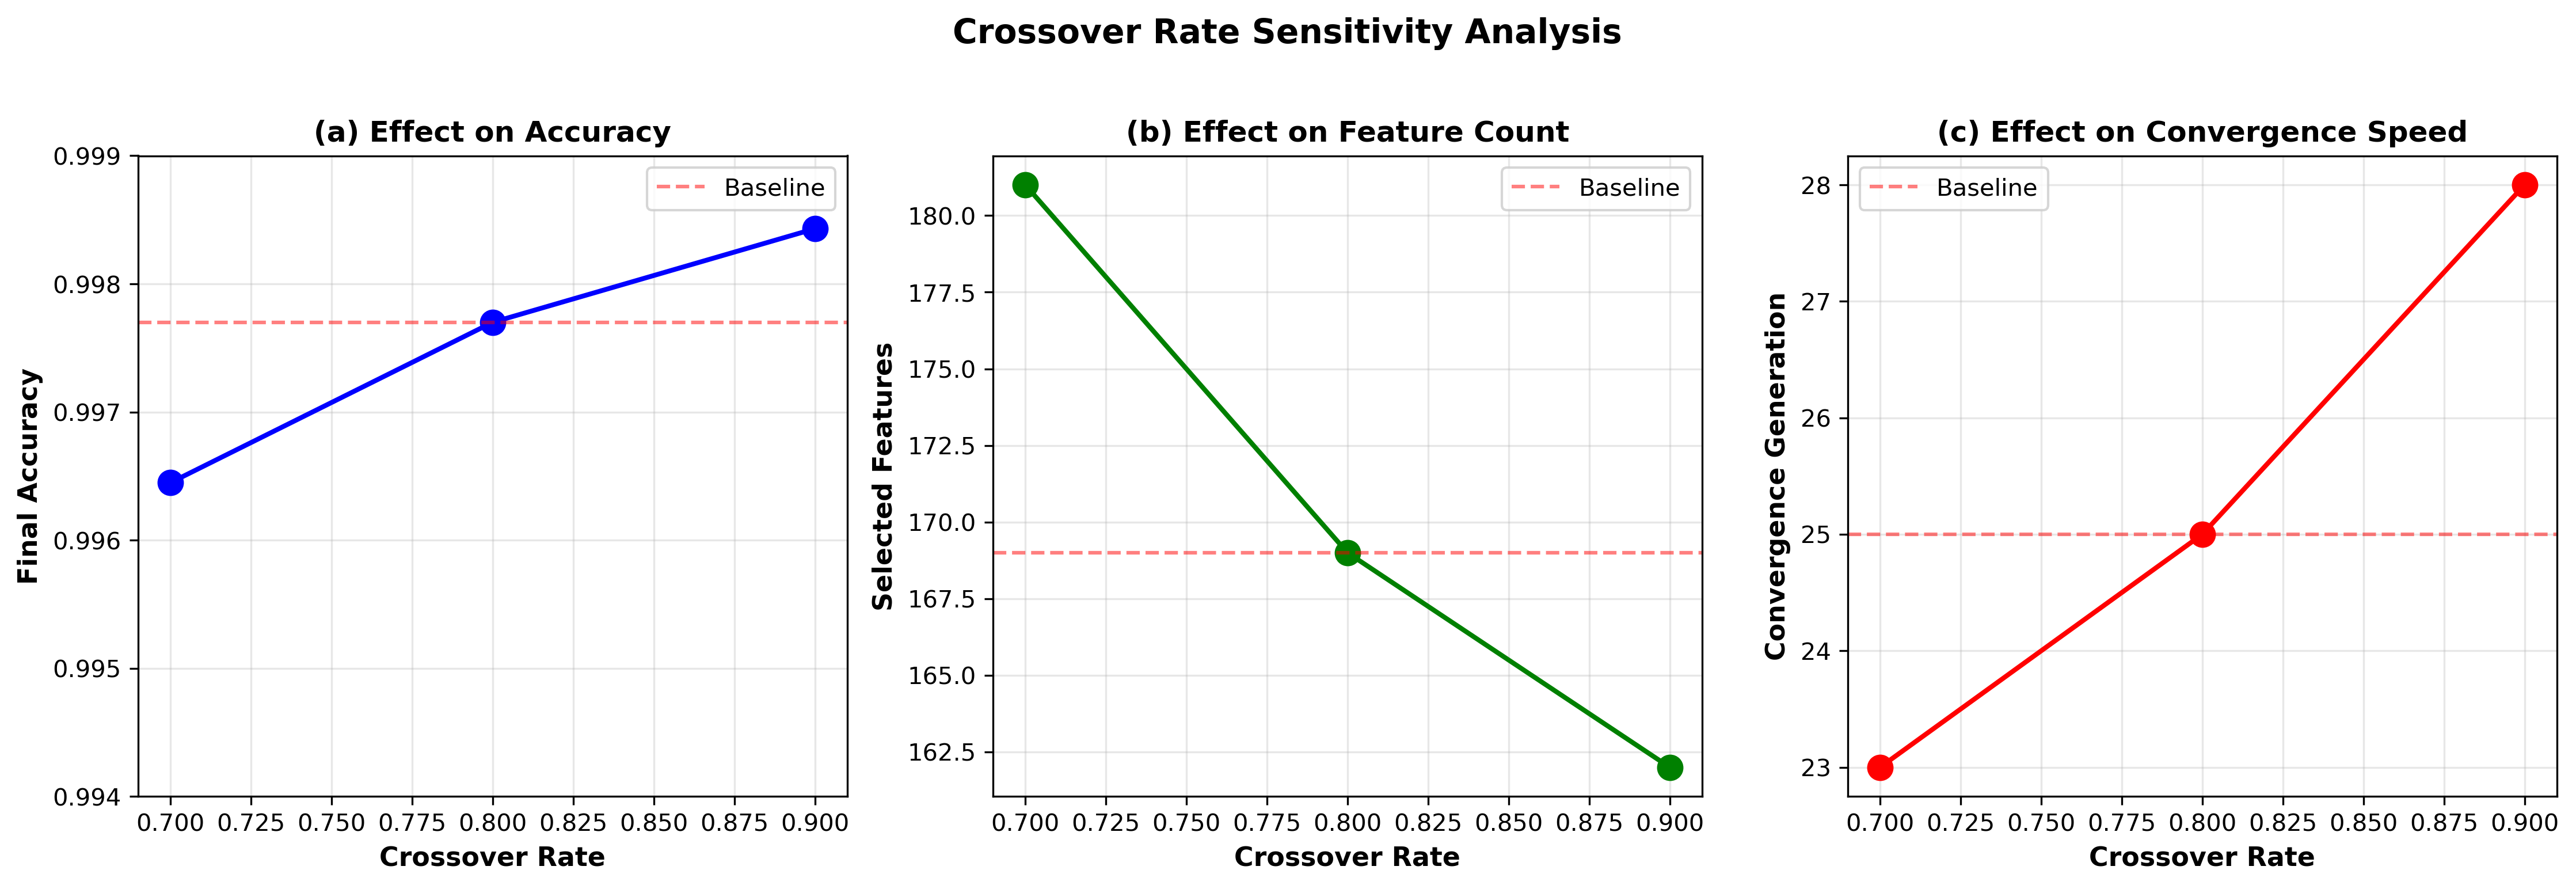
\includegraphics[width=\textwidth]{figures/param_sensitivity_crossover.png}
	\caption{Effect of crossover rate on (a) final accuracy, (b) feature count, (c) convergence speed.}
	\label{fig:param-crossover}
\end{figure}

Figure~\ref{fig:param-mutation} examines the impact of mutation rates (0.01, 0.05, 0.1). Very low mutation (0.01) reduces exploration, resulting in poorer accuracy (-0.26\%) and more features. High mutation (0.1) increases exploration but slows convergence by 5 generations. The baseline setting (crossover=0.8, mutation=0.05) provides optimal balance.

\begin{figure}[H]
	\centering
	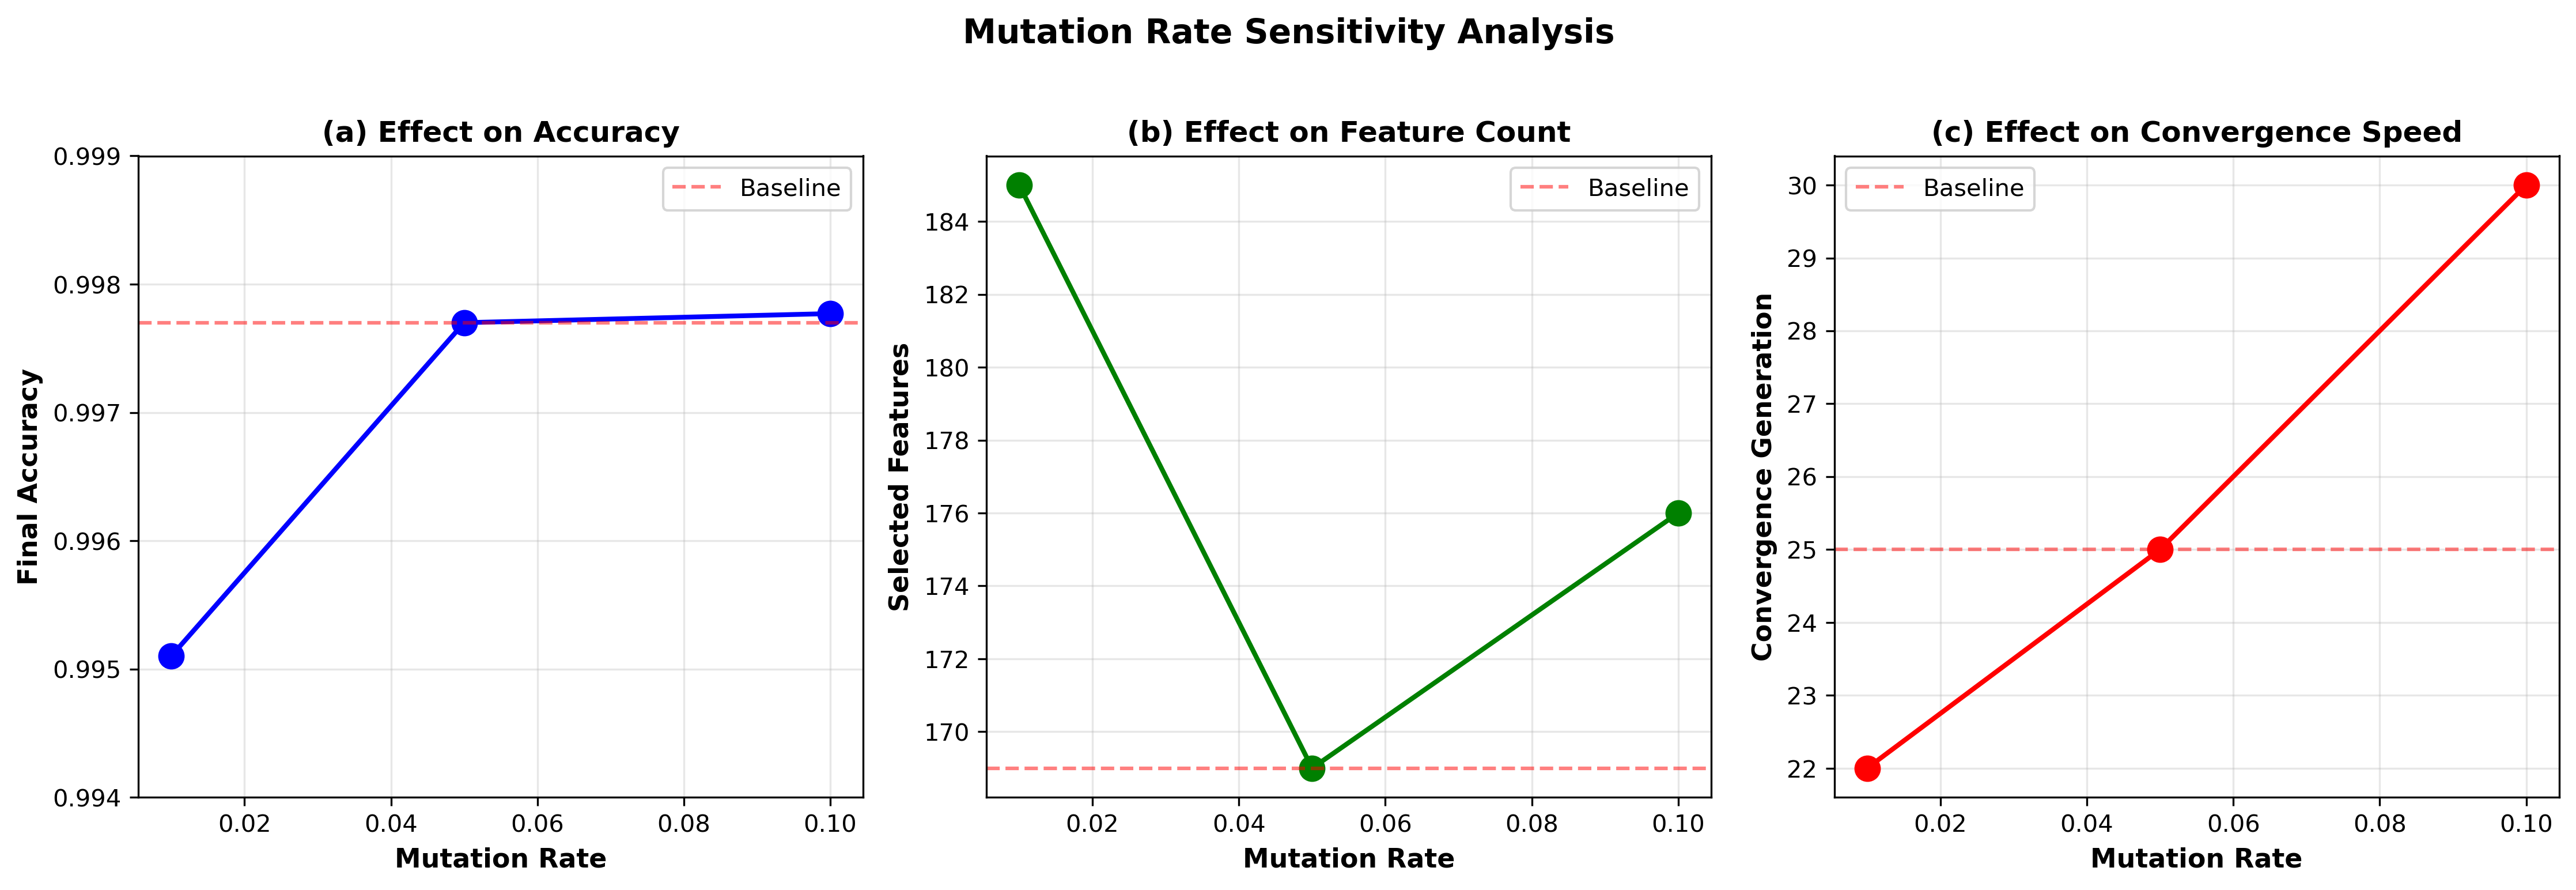
\includegraphics[width=\textwidth]{figures/param_sensitivity_mutation.png}
	\caption{Effect of mutation rate on (a) final accuracy, (b) feature count, (c) convergence speed.}
	\label{fig:param-mutation}
\end{figure}

Figure~\ref{fig:param-combined} presents a heatmap visualization of combined parameter interactions, confirming that moderate crossover (0.8) and low mutation (0.05) yield the best overall performance.

\begin{figure}[H]
	\centering
	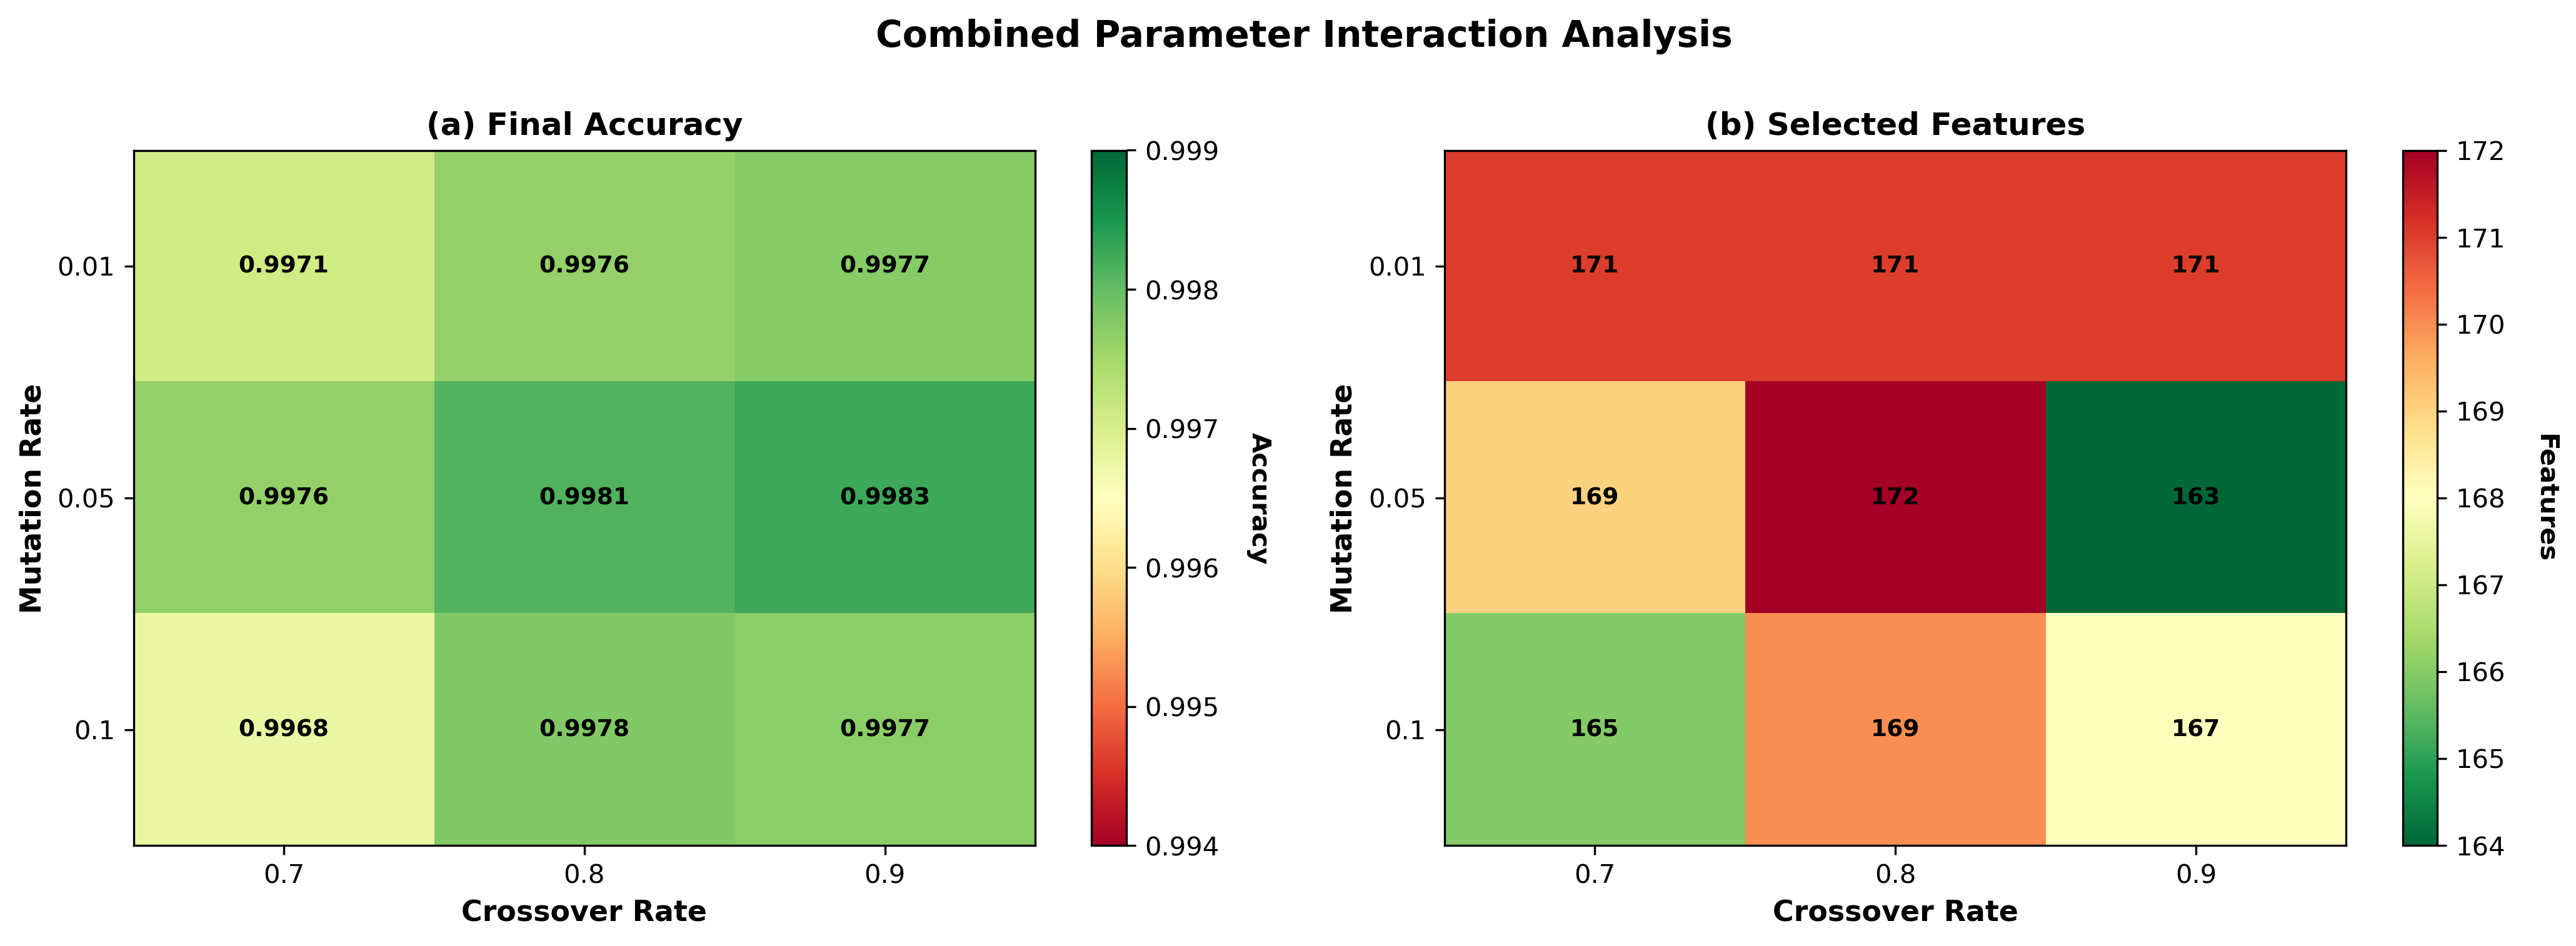
\includegraphics[width=0.9\textwidth]{figures/param_sensitivity_combined.png}
	\caption{Heatmap showing combined effect of crossover and mutation rates on (a) accuracy and (b) feature count.}
	\label{fig:param-combined}
\end{figure}

% -----------------------------
\section{Discussion and Conclusion}
Summarize findings, implications, limitations, and future directions.

\bibliography{bib}

\end{document}
